\documentclass[10pt,a4paper]{article}

\usepackage[margin=1.65cm]{geometry}
\usepackage[T1]{fontenc}
\usepackage{lmodern}
\usepackage{amsmath,amssymb}
\usepackage{graphicx}
\usepackage{booktabs}
\usepackage{microtype}
\usepackage[hidelinks]{hyperref}
\usepackage[font=small,labelfont=bf]{caption}
\usepackage{titlesec}

\titleformat{\section}
  {\normalsize\bfseries}{\thesection}{0.5em}{}
\titlespacing*{\section}{0pt}{8pt}{4pt}

\setlength{\parindent}{0pt}
\setlength{\parskip}{4pt}
\setlength{\textfloatsep}{8pt}
\setlength{\intextsep}{8pt}
\setlength{\abovecaptionskip}{4pt}

\begin{document}

\begin{center}
    {\Large\bfseries Accelerating Total-Variation Image Denoising}\\[4pt]
    Alexandros Vryonides\\
    EEP55C36 --- Computational Methods and Algorithms
\end{center}

\section{Problem and reproduction scope}

I compared Chambolle's fixed-point TV denoising method with accelerated projected dual gradients. The baseline follows the course guide's
two-dimensional isotropic formulation.
A no-momentum projected solver isolates acceleration's contribution.
All methods minimize the same objective.

I tested whether acceleration reduces runtime to a shared optimization
tolerance without materially changing reconstruction quality.

Let $u,f\in\mathbb{R}^{H\times W}$ denote the clean and observed
grayscale images. The observation model is
$f_{ij}=u_{ij}+\epsilon_{ij}$, where the noise values are independent
and $\epsilon_{ij}\sim\mathcal{N}(0,\sigma^2)$.
Pixel intensities are dimensionless; clean intensities lie in $[0,1]$.
Noisy observations and reconstructions are not clipped.

For a reconstruction $v$, the objective is
\begin{equation}
 P(v)=\frac12\|v-f\|_F^2+\lambda\,\mathrm{TV}(v),
 \qquad
 \mathrm{TV}(v)=
 \sum_{i,j}\sqrt{(D_1v)_{ij}^{\,2}+(D_2v)_{ij}^{\,2}}.
 \label{eq:objective}
\end{equation}
Here $D_1$ and $D_2$ are vertical and horizontal forward differences,
with zero differences on the final row and final column respectively.
The squared Frobenius norm sums squared entries.
The parameter $\lambda>0$ controls regularization strength.

TV favours piecewise-constant images but can suppress genuine texture.
The strictly convex data term ensures a unique minimizer, not
suitability for every image.

\section{Baseline, modification and verification}

The auxiliary field $p=(p_1,p_2)$ contains two arrays of shape
$H\times W$. Divergence satisfies
$\langle\nabla v,p\rangle=-\langle v,\operatorname{div}p\rangle$,
fixing the signs and boundary treatment.

Starting from $p^0=0$, Chambolle's baseline computes
\begin{equation}
 g^k=\nabla\!\left(\operatorname{div}p^k-f/\lambda\right),
 \qquad
 p^{k+1}_{ij}=
 \frac{p^k_{ij}+\tau g^k_{ij}}
      {1+\tau\|g^k_{ij}\|_2},
 \qquad \tau=\frac18.
 \label{eq:baseline}
\end{equation}
The reconstruction is $v^{k+1}=f-\lambda\operatorname{div}p^{k+1}$.
All vector norms and divisions in the update are evaluated per pixel.

The modification instead takes a projected gradient step from an
extrapolated field $y^k$:
\begin{equation}
 a^k=y^k+\frac18\nabla\!\left(\operatorname{div}y^k-f/\lambda\right),
 \qquad
 p^{k+1}_{ij}=\frac{a^k_{ij}}{\max(1,\|a^k_{ij}\|_2)}.
 \label{eq:projection}
\end{equation}
With $t_0=1$ and $y^0=p^0=0$, momentum is
\begin{equation}
 t_{k+1}=\frac{1+\sqrt{1+4t_k^2}}2,\qquad
 \beta_k=\frac{t_k-1}{t_{k+1}},\qquad
 y^{k+1}=p^{k+1}+\beta_k(p^{k+1}-p^k).
\end{equation}
Setting $\beta_k=0$ gives the no-momentum ablation.
The feasible field $p$, not the extrapolated field $y$, is used for
reconstruction and convergence checks.

For $q=\lambda\operatorname{div}p$, a feasible field
$\|p_{ij}\|_2\leq1$ gives the dual lower bound
$D(p)=\langle f,q\rangle-\frac12\|q\|_F^2$.
I stop when
\begin{equation}
 \frac{P(v)-D(p)}{\max(1,|P(v)|,|D(p)|)}\leq10^{-3}.
 \label{eq:gap}
\end{equation}
The gap is checked every ten iterations and at the shared cap of
20\,000 iterations. Non-finite or significantly negative normalized
gaps raise errors. Fixed-count runs remain available for verification.
Each solver has $O(HW)$ work per iteration and $O(HW)$ storage;
momentum adds array operations and storage.

The 29 tests cover exact updates, adjointness, feasibility, boundaries
and input/mean preservation. All solvers recover the known optimum
$[0.2,0.8]$ for $f=[0,1]$ and $\lambda=0.2$.

\newpage

\section{Experimental design}

Synthetic $96\times96$ images contain four rectangles and two disks.
A stress variant replaces the central region with a checkerboard of
intensities 0.4 and 0.6 and two-pixel squares. Noise levels are
$\sigma\in\{0.05,0.10,0.20\}$.
Development smoke cases used seeds 0 and 1, validation used seeds
100--109, and final testing used seeds 1000--1019.
TV denoising requires no supervised offline training.

Validation selected $\lambda=0.175$ by minimizing mean MSE across
30 cases, using accelerated solves at gap tolerance $10^{-5}$.
The candidate grid was extended after its initial winner reached
the upper endpoint. The selected value was frozen before final testing.

Two low-noise development cases exceeded the original 5000-iteration
cap, motivating a shared cap of 20\,000 at unchanged tolerance.
Initial results and corrections appear in
\texttt{docs/overall\_assessment.md}.

Final evaluation contains 20 paired cases per noise level and image
type: 120 image/noise cases and 360 method-case results.
Every method receives identical observations and permitted information.
All final runs reached the specified tolerance.

The primary outcome is paired runtime saving at matched gap tolerance.
Secondary outcomes are iterations, MSE and peak signal-to-noise ratio
(PSNR). For $N=HW$ pixels,
\[
 \mathrm{MSE}=\frac1N\sum_{i,j}(v_{ij}-u_{ij})^2,
 \qquad
 \mathrm{PSNR}=10\log_{10}(1/\mathrm{MSE}).
\]
MSE is also measured within the checkerboard region.
Lower MSE and higher PSNR indicate better reconstruction.

I calculated percentile bootstrap 95\% confidence intervals using
10\,000 resamples of whole paired seed cases within each condition
(analysis seed 2026). Pixels and timing repetitions are not independent
cases; conditions sharing seeds are analysed separately.

\section{Runtime results and ablation}

Figure~\ref{fig:speed} reports mean case-level reference-to-accelerated
runtime ratios. All conditions favour acceleration: runtime-saving
intervals exceed zero and speedup intervals exceed one.

\begin{figure}[htbp]
 \centering
 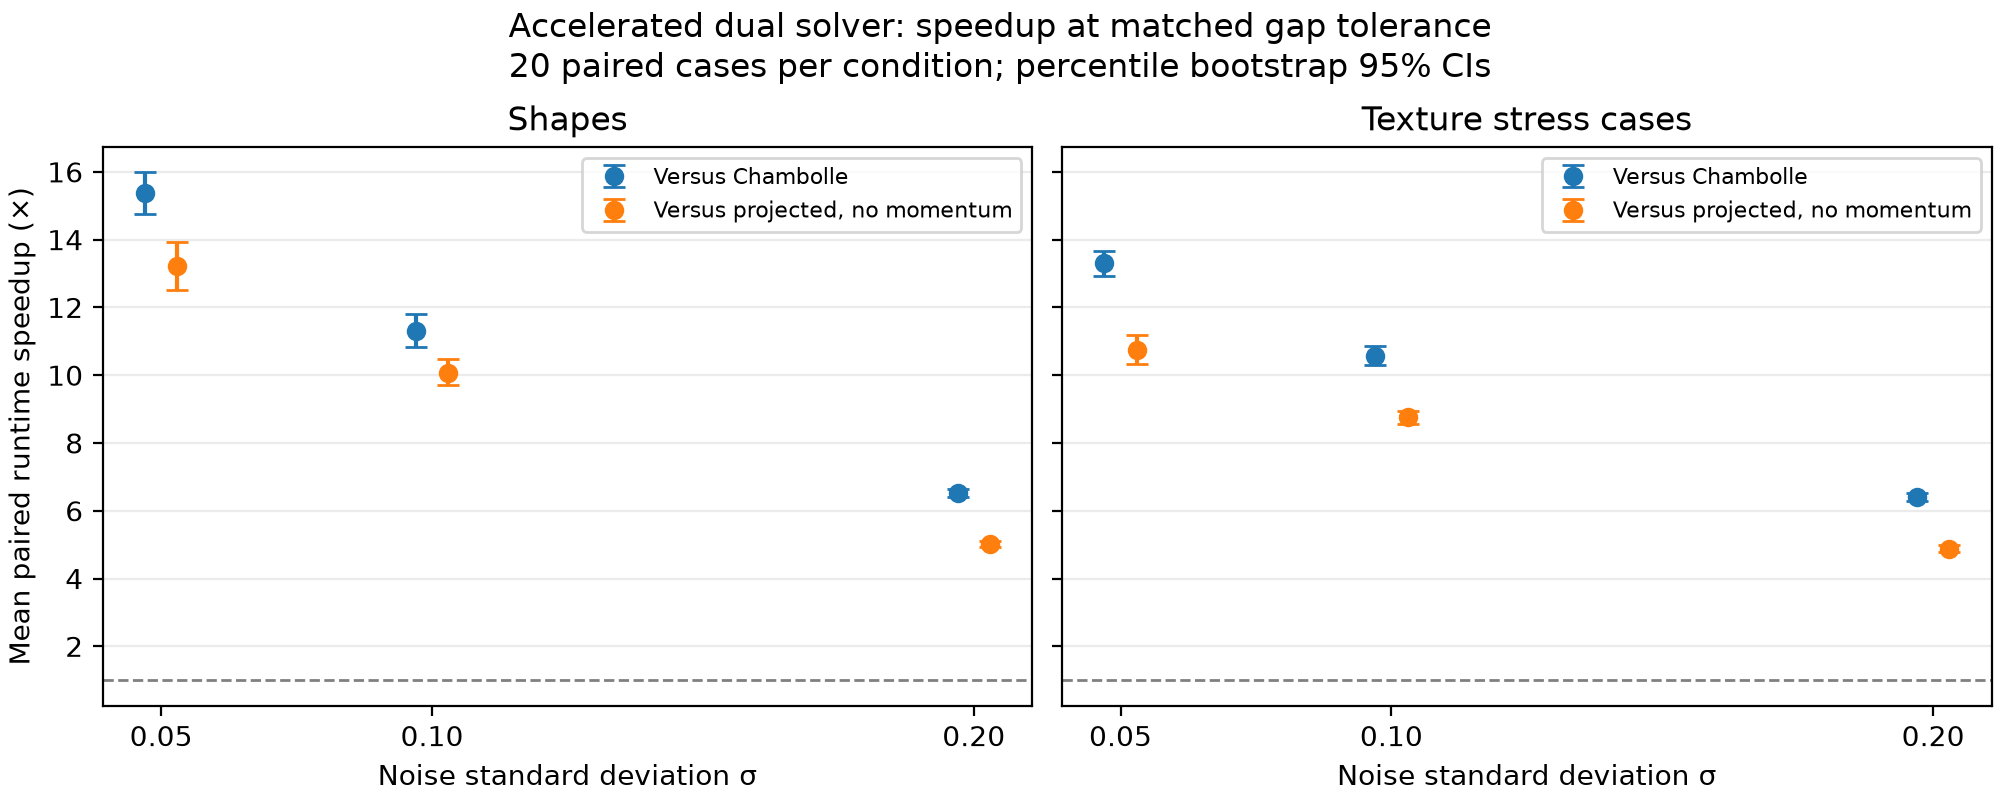
\includegraphics[width=0.85\linewidth]{figures/runtime_speedup.png}
 \caption{Acceleration reduces runtime relative to both Chambolle and
 the no-momentum projected solver. Error bars are paired bootstrap
 95\% confidence intervals.}
 \label{fig:speed}
\end{figure}

Mean speedup over Chambolle was $6.41$--$15.38\times$.
For shapes, speedup decreased from $15.38\times$ at $\sigma=0.05$
(95\% CI $14.75$--$15.98$) to $6.53\times$ at $\sigma=0.20$
($6.41$--$6.65$). Acceleration also exceeded the no-momentum solver
by $4.88$--$13.22\times$, supporting momentum's contribution.
\newpage

\section{Reconstruction quality and limitations}

\begin{figure}[htbp]
 \centering
 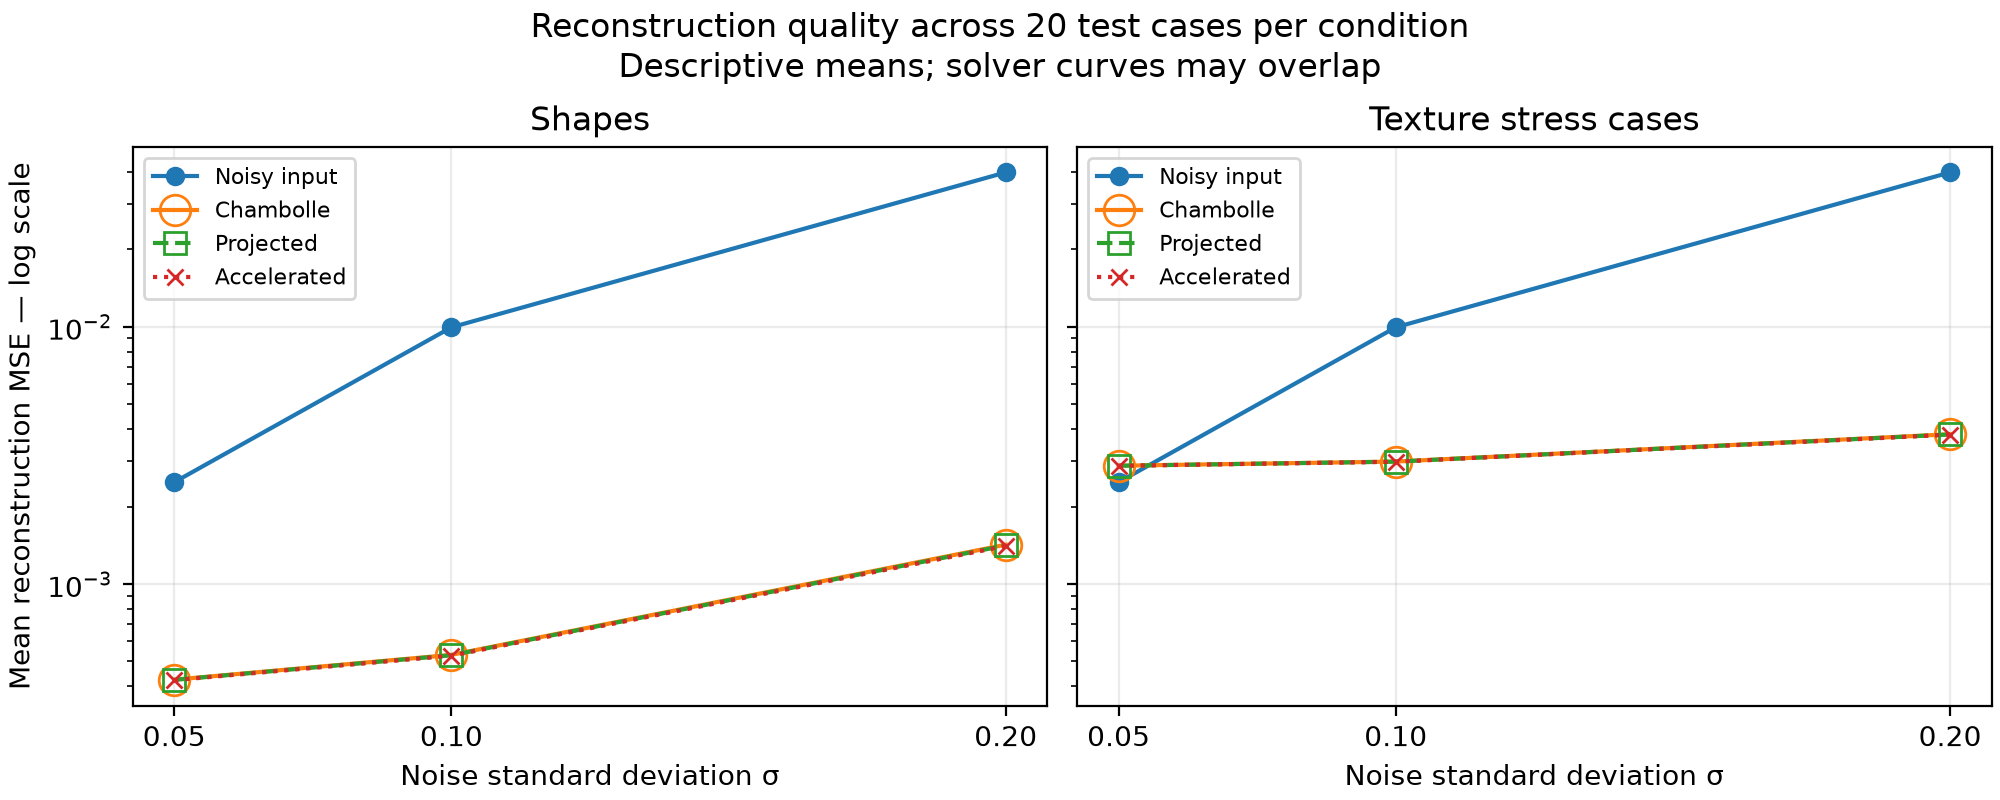
\includegraphics[width=0.85\linewidth]
 {figures/reconstruction_quality.png}
 \caption{Mean MSE across 20 cases per condition, with a logarithmic
 vertical axis. Solver curves nearly overlap. These are descriptive
 means, without uncertainty bars.}
 \label{fig:quality}
\end{figure}

Reconstruction MSE nearly overlaps across solvers
(Figure~\ref{fig:quality}). For shapes at $\sigma=0.10$, mean MSE
was $0.00053052$ for Chambolle and $0.00052646$ for acceleration.
Small differences reflect approximate stopping, not a changed prior.

The fixed example (seed 1000, $\sigma=0.10$;
Figure~\ref{fig:examples}) shows noise suppression and broad-shape
preservation, alongside softened boundaries and lost checkerboard texture.


\begin{figure}[htbp]
 \centering
 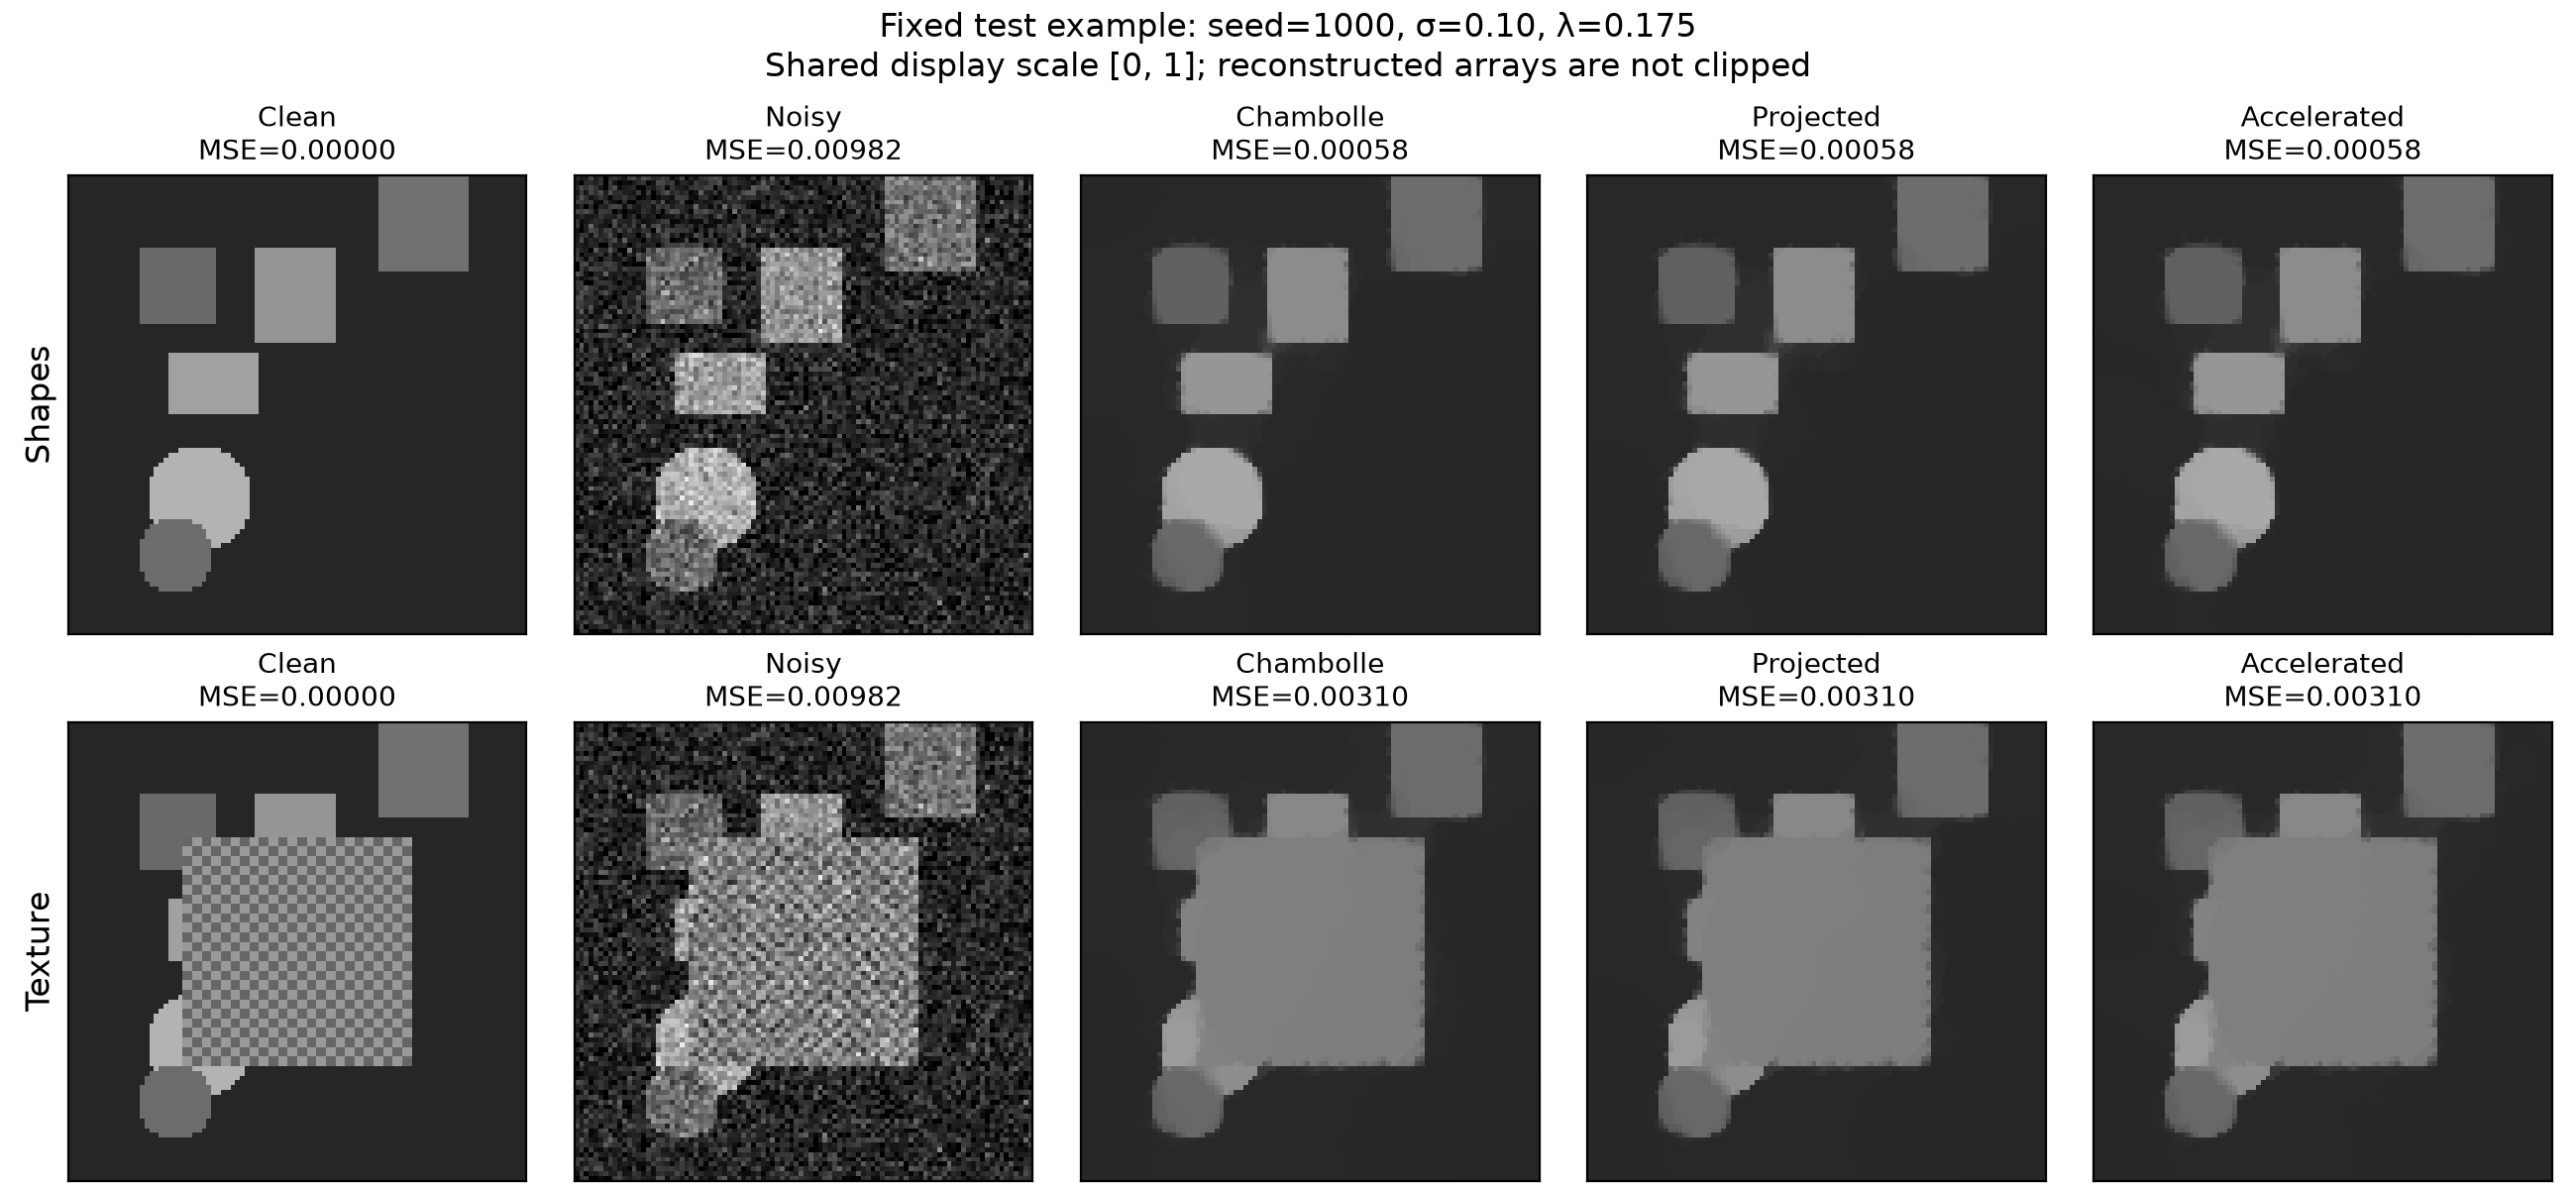
\includegraphics[width=0.85\linewidth]
 {figures/reconstruction_examples.png}
 \caption{Fixed shapes and texture examples. All panels share display
 limits $[0,1]$; numerical arrays are unclipped. The similar outputs
 demonstrate both matched reconstruction quality and shared texture loss.}
 \label{fig:examples}
\end{figure}

The stress result distinguishes optimization accuracy from task quality.
At $\sigma=0.05$, mean noisy-image MSE was approximately $0.0025$,
whereas denoised texture MSE was approximately $0.00288$.
The accelerated method's checkerboard-region MSE was approximately
$0.00996$. All runs converged, but genuine texture was penalized
alongside noise.

Acceleration reduced runtime with similar MSE in this synthetic study.
Results are limited to one machine, small images and Gaussian noise.
A shared $\lambda$ can oversmooth texture; momentum overhead may limit
benefits on easy problems. Confidence intervals describe case variation
within each condition, not hardware variation or simultaneous coverage.

\section{Reproduction and contribution}

Repository:
\url{https://github.com/AVryonides/tv-denoising}.
The README documents installation, verification, experiment and
figure-generation commands.

\textbf{Assistance.}
ChatGPT assisted with explanations, generated and corrected code,
tests, experiments, analysis and writing. Full attribution and
development history are recorded in the repository.

\noindent\textbf{References:}
\href{https://github.com/AVryonides/tv-denoising#references}
{Full references in the project repository}.

\end{document}